\documentclass[a4paper, 11pt]{scrartcl}

%Packages
\usepackage[left=2cm,right=3cm,top=3.4cm,bottom=3cm]{geometry}
\usepackage[utf8]{inputenc}
\usepackage[ngerman]{babel}
\usepackage[T1]{fontenc}
\usepackage{color}
\usepackage{xcolor}
\usepackage{fontspec}
\usepackage[ddmmyyyy]{datetime}
\usepackage{tabto}
\usepackage[headsepline]{scrlayer-scrpage}
\usepackage{ragged2e}
\usepackage{ulem}
\usepackage{hyperref}
\usepackage{soul}
\usepackage{graphicx}
\usepackage{setspace}
\usepackage{stix}

\setmainfont{Calibri}
\color{black}
\renewcommand{\dateseparator}{.}
\graphicspath{ {./img/} }
\setcounter{tocdepth}{1}

%Colors
\definecolor{grey}{HTML}{1A1A1A}
\definecolor{heading}{HTML}{5B9BD5}
\definecolor{color-section}{HTML}{2D74B5}
\definecolor{light-grey}{HTML}{888888}
\definecolor{grey-blue}{HTML}{44536A}

%fonts
\setkomafont{section}{\normalfont\fontsize{14}{1}\fontspec[Ligatures=TeX]{Calibri Light}\color{color-section}}
\setkomafont{subsection}{\normalfont\fontsize{13}{1}\fontspec[Ligatures=TeX]{Calibri Light}\color{color-section}}

\begin{document}
	\ofoot{\pagemark}
	\cfoot{}
	\begin{titlepage}
		\color{heading}
	 	\begin{flushleft}
			{\fontsize{28}{10}\fontspec[Ligatures=TeX]{Calibri Light}Textverarbeitung} \\
			\color{black} {Ein Leitprogramm}

	  	\vfill
	  	
					 Name:   	   \hspace{2mm} Luca \\
		\vspace{2mm} Datum:  	   \hspace{1mm} \today \\ % aktuelles Datum
		\vspace{5mm} Klasse: 	   \hspace{2mm} 11BG-PI2 \\
		\vspace{10mm} Fach:   	   \hspace{14mm} Technische Kommunikation \\
					 Fachlehrer:   \hspace{5mm} Danilo Magdeburg, Elisabeth Engel
		\end{flushleft}
	\end{titlepage}
	\ihead{\normalfont\fontsize{11}{1}\fontspec[Ligatures=TeX]{Calibri}\color{black}Luca Florian Halbich}
	\chead{\normalfont\fontsize{11}{1}\fontspec[Ligatures=TeX]{Calibri}\color{black}Textverarbeitung}
	
	\tableofcontents
	
	\pagenumbering{roman}
	\newpage
	\section{Einführung und Aufbau} %Beginn Kapitel 1 Einführung und Aufbau
	\pagenumbering{arabic}
	\setcounter{page}{1}
	\ifoot{\normalfont\today}
	\begin{justify} \fontsize{11}{5}
		Bei der Erstellung des Dokumentes geht es darum Textverarbeitung zu üben. Das Dokument ist ausschließlich geeignet für Teilnehmer der Veranstaltung „Technische Kommunikation“. Denn dieses Dokument kann und soll als Basisdokument für Ihre schulischen Ausarbeitungen genutzt werden.\vspace{2mm} \\
		Wer das vorliegende Dokument eigenständig erstellt hat, sollte in der Lage sein, Office- Dokumente für die Schule und später auch Studium zu erstellen. Um richtig fit zu sein, braucht es allerdings noch viel mehr Übung, und sicherlich auch viele Hinweise aus dem Internet ;) .\vspace{2mm} \\
		Dieses Dokument dient als Leitprogramm ist wie folgt aufgebaut: \vspace{2mm} \\
		Innerhalb der jeweiligen Kapitel werden verschiedenen Funktionen von Microsoft Word respektive Libre / Open Office Writer behandelt, welche Sie anschließend umsetzen sollen. Beginnend bei der Formatierung, über Absätze, Formatvorlagen, Seitenlayout, Grafiken, Tabellen bis hin zu Verzeichnissen. Wie die jeweiligen Funktionen umgesetzt werden, entnehmen Sie den entsprechenden Anleitungen$^{1}$ auf Moodle. Innerhalb des Kapitels steht zudem die Referenz zu den jeweiligen Kapiteln / Seiten der Anleitungen$^{2}$, sodass Sie im Selbststudium die verschiedenen Funktionen Ihrer Textverarbeitungssoftware kennenlernen. Dieses Dokument lehnt sich verstärkt an das Dokument von Alker et al. (vgl. 2019) an, weswegen mehrere Direktzitate verwendet werden. Die Informationen lassen sich eins-zu-eins auf LibreOffice / OpenOffice übertragen. \vspace{2mm} \\
		Ihre Aufgabe ist es nun, die Inhalte auf Ihre „Start“-Datei zu übertragen und kapitelweise abzugeben. Dabei wird es zwangsläufig passieren, dass nicht alle Seiten direkt richtig formatiert sind. Dies ist nicht weiter schlimm, wenn es nicht direkt wie die Vorlage aussieht. Beispielsweise kommt das Kapitel Inhaltsverzeichnis (vgl. Kap. 8 ) relativ spät, weswegen jenes, aufgrund der Vergleichbarkeit, bei früheren Abgaben nicht bearbeitet werden soll respektive muss. Ziel ist nur, dass Sie die einzelnen Inhalte der Kapitel umsetzen. Sollte Ihr Ergebnis nicht genau wie die Vorlage aussehen, ist dies nicht weiter schlimm, da beide Textverarbeitungsprogramme meist kleine Unterschiede in der Art der Formatierung aufweisen. \vspace{2mm} \\
		Abschließend wird ein beispielhafter Aufbau einer Projektdokumentation dargestellt, welchen Sie für zukünftige Ausarbeitungen nutzen können. \vspace{2mm} 		
	\end{justify}
	\begin{flushleft}
		Abgaben, welche für einen 90 Minuten-Block vorgesehen sind:
		\begin{itemize}
			\item Kapitel 2 – Formatierung \\ Kapitel 3 – Absätze \vspace{3mm}
			\item Kapitel 4 – Formatvorlagen \\ Kapitel 5 – Seitenlayout \vspace{3mm}
			\item Kapitel 6 – Kopf- und Fußzeile \\ Kapitel 7 – Tabellen \\ Kapitel 8 – Verzeichnisse
		\end{itemize}
	\end{flushleft}
	
	\vfill
		
	\begin{justify}			
		\rule{50.8mm}{0.3mm} \\
		\small
		$^{1}$ \hspace{2mm} Wies, P. (2014): OpenOffice Writer 4 / LibreOffice Writer 4. Herdt Verlag. Bodenheim. \\ \hspace{3mm} Alker, T./ Spieß, S./ von Braunschweig, C. (2019): Word 2019 Grundlagen. Herdt Verlag. Bodenheim. \vspace{2mm} \\
		$^{2}$ \hspace{2mm} Für die bessere Lesbarkeit werden die Referenzen in Form (vgl. 6; 9) angegeben. \\ Die erste Zahl stellt die Seite für das Dokument von LibreOffice dar. Letztere hingegeben für Microsoft Word.
	\end{justify}
	%Ende Kapitel 1 Einführung und Aufbau
	
	\newpage
	\section{Formatierung} %Beginn Kapitel 2 Formatierung
	\begin{justify}
		Jede Textverarbeitungssoftware gibt uns die Möglichkeit einem Text eine Zeichenformatierung zuzuweisen (vgl. 40-41; 30-31) und beeinflusst maßgeblich das Aussehen Ihres Dokuments (vgl. Alker et al. 2019: 29). Dies dient dazu, um den Blick des Lesers auf bestimmte Informationen zu lenken. Beachten Sie, dass Sie Text mit maximal zwei Zeichenformatierungen belegen. Alles darüber wirkt unprofessionell.
	\end{justify}
	\begin{flushleft}
		So gibt es die Möglichkeit den Text in Calibri oder alternativ {\normalfont\fontspec[Ligatures=TeX]{Arial}Arial} \vspace{2mm} \\
		\textbf{Fett gedruckt} \vspace{2mm} \\
		\underline{Unterstrichen} \vspace{2mm} \\
		\textit{kursiv} \vspace{2mm} \\
		\sout{durchgestrichen} \vspace{2mm} \\
		{\normalfont\fontspec[Ligatures=TeX]{Courier New}in einer anderen Schriftart (Courier New)} \vspace{2mm} \\
		als Link \url{https://de.libreoffice.org/get-help/documentation} \\
		(Einfügen --> Hyperlink) \vspace{8mm} \\
		{\color{red}farbig} \vspace{2mm} \\
		Hoch$^{gestellt}$ und Tief$_{gestellt}$ \vspace{2mm} \\
		in {\Large Schriftgröße 14} und {\scriptsize Schriftgröße 8} \vspace{2mm} \\
		\hl{zu gestalten}.
	\end{flushleft}
	%Ende Kapitel 2 Formatierung
	
	\newpage
	\section{Absätze} %Beginn Kapitel 3 Absätze
	\begin{justify}
		Als Absatz wird ein Bereich bezeichnet, der mit einer Absatzschaltung (Enter) beendet wurde. Damit wird die Zeile umgebrochen und ein neuer Absatz beginnt. Die Absatzformatierung betrifft u. a folgende Gestaltungsaspekte (Alker et al. 2019: 40):
		\begin{itemize}
			\setlength\itemsep{0.001em}
			\item \textbf{Ausrichtung:} Ein Absatz lässt sich beispielsweise zentriert oder im Blocksatz ausrichten.
			\item \textbf{Zeilenabstände} definieren den Abstand der Zeilen innerhalb des Absatzes.
			\item \textbf{Absatzabstände:} Vor und nach dem Absatz lassen sich feste Abstände definieren.
			\item \textbf{Absatzeinzüge:} Sie können Einzüge von links und rechts definieren. Auch können Sie Zeilen eines Absatzes einrücken.
			\item Nummerierungen/Aufzählungen
			\item Schattierungen und Rahmen
		\end{itemize}
		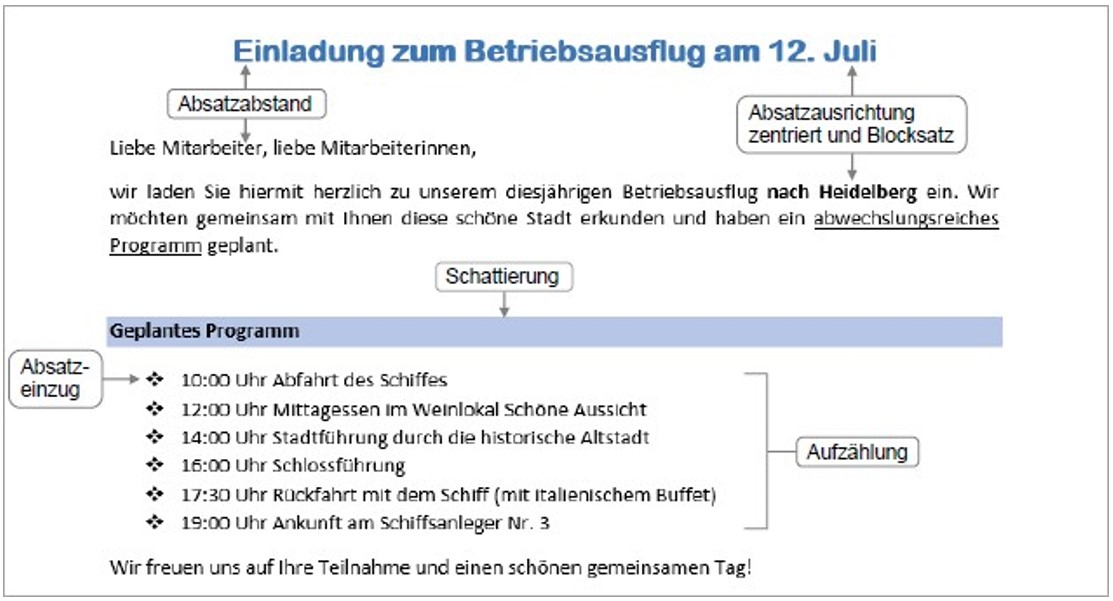
\includegraphics[width=13.44cm, height=7.2cm]{Abbildung01}\\
		{\normalfont\scriptsize\color{grey-blue}\textit{Abbildung 1: Absätze}}
	\end{justify}
	\subsection*{Ausrichtung}
	Absätze können dazu (vgl. 46; 41):\\
	\makebox[\textwidth]{Zentriert} \\
	Linksbündig \\
	\begin{flushright}
		\vspace{-7mm}
		Rechtsbündig ausgerichtet werden.
	\end{flushright}
	\begin{justify}
		\vspace{-2mm}
		Bei längeren Fließtexten (und generell für Ausarbeitungen) eignet sich der Blocksatz, da die Ausarbeitung somit ein einheitliches Bild wiedergibt. Dabei „wird der Text am linken und am rechten Seitenrand ausgerichtet, wobei zwischen den Wörtern so viel zusätzlicher Leerraum eingefügt wird, bis die Zeile beide Seitenränder erreicht. Um diesen Leerraum zu verkleinern, hilft oft die Silbentrennung“ (Alker et al. 2019: 41).
	\end{justify}
	\subsection*{Absatzabstand}
	\begin{justify}
		Insbesondere bei Überschriften oder auch Aufzählungen, sollte mit dem Absatzabstand gearbeitet werden (vgl. 46; 42). \vspace{2.5mm} \\
		Jener hilft ein einheitliches Bild mit immer gleichen Abständen vor und nach einem Textblock zu schaffen, ohne dass der Nutzer beliebig viele Leerzeilen mit unterschiedlicher Schriftgröße einfügen muss.
	\end{justify}
	\subsection*{Zeilenabstand}
	\begin{justify}
		\setstretch{1.05}
		Beim Zeilenabstand handelt es sich um den Abstand der einzelnen Zeilen innerhalb eines Absatzes. Einen Absatz mit mehreren Zeilen erhalten Sie immer dann, wenn Sie am Ende einer Zeile weitertippen, ohne Enter zu betätigen, sodass die Software den Text automatisch in einer neuen Zeile weiterführt. Standardmäßig beträgt der Zeilenabstand 1,08 (vgl. 46; 43). \vspace{2,5mm} \\
		Einige Lehrer oder später auch Dozenten bzw. Professoren verlangen einen Abstand von 1,5. Mit dem Hintergrund, dass sich jener Abstand dazu eignet eigene Anmerkungen zu ergänzen. Welcher Abstand jedoch verlangt wird, erfragen Sie bitte vorab bei der betreuenden Person.
	\end{justify}
	\subsection*{Aufzählung und Nummerierung}
	Hierbei gibt es (vgl. 48; 43):\\
	\begin{itemize}
		\vspace{-6mm}
		\setlength\itemsep{0.01mm}
		\item Aufzählung
		\item Nummerierung \\
	\end{itemize}
	Dabei ist es möglich, das entsprechende Aufzählungs-, bzw. Nummerierungsformat zu ändern.\\
	\begin{itemize}
		\vspace{-6mm}
		\setlength\itemsep{0.01mm}
		\item[-] Aufzählung 1
		\item[-] Aufzählung 2
		\vspace{4mm}
		\item Aufzählung 1
		\item Aufzählung 2
		\vspace{4mm}
		\item[1.] Aufzählung 1
		\item[2.] Aufzählung 2
		\vspace{4mm}
		\item[a.] Aufzählung 1
		\item[b.] Aufzählung 2
		\vspace{4mm}
	\end{itemize}
	\begin{justify}
		Es gibt aber auch die Möglichkeit in die Tiefe zu gehen (vgl. 50, 45). Nutzen Sie dafür die Schaltfläche für Einzug vergrößern / verkleinern oder auch die Tabulatortaste bzw. Shift+Tabulator. Tabulatoren sind feste Positionen innerhalb einer Zeile, die über die T-Taste mit dem Cursor angesprungen werden. Dies ist z. B. beim Erstellen von tabellarischen Listen sehr praktisch (Wies 2014: 51).
	\end{justify}
	\begin{itemize}
		\item Ebene 1
		\begin{itemize}
			\item[$\circ$] Ebene 2
			\item[$\circ$] Ebene 2
			\begin{itemize}
				\item[$\smblksquare$] Ebene 3
			\end{itemize}
			\item[$\circ$] Ebene 2 \\
			Wenn Sie einen Zeilenumbruch innerhalb einer Nummerierung erzwingen wollen, drücken Sie Shift + Enter. So erzeigen Sie einen weichen Umbruch.
			\item[$\circ$] Ebene 2
			\item[$\circ$] Ebene 2
		\end{itemize}
	\end{itemize}
	\newpage
	\subsection*{Formatierungszeichen}
	\begin{justify}
		Es kommt manchmal vor, dass Ihr Textverarbeitungsprogramm nicht so agiert, wie Sie wollen. Dies hängt meist mit Absatzmarken zusammen, welche im „Normalbetrieb“ unsichtbar sind. Um zu erkennen, wo Tabstopps oder Leerzeichen eingesetzt worden sind, drücken Sie auf ¶ (vgl. 51; 48).
	\end{justify}
\end{document}























